\documentclass{article}

\usepackage{amsmath}
\usepackage{amssymb}
\usepackage{graphicx}
\usepackage{tikz}
\usetikzlibrary{arrows}
\usepackage{verbatim}
\usepackage{sfmath}
\usepackage{psfrag}
\usepackage{here} 
\usepackage{hyperref}
\usepackage{xcolor}
\usepackage{tcolorbox}


%\textheight=24cm

%\renewcommand\sfdefault{phv}     %use helvetica for sans serif
\renewcommand{\familydefault}{\sfdefault}
\renewcommand{\familydefault}{cmss}

\begin{document}

\begin{center}
\bf{\huge 
Ingenier\'{\i}a de Control\\
\vspace{0.25cm}
Pr\'actica 2
}
\end{center}

\section*{Aircraft vertical takeoff and landing}

Consider the simplified planar model of the system for vertical takeoff and landing of an aircraft represented in Figure~\ref{fig:figure_2}, in which the aircraft is represented by a bar. 
The position of the center of mass of the aircraft, $\mathbf{c} =  (x, y)^T$, the roll angle of the aircraft, $\theta$, and their time derivatives are the state variables of the system.  
The thrust force $S$, applied to the center of mass of the aircraft, and the forces $F$, applied to the wing tips, are the control inputs $u_1$ and $u_2$ of the system, respectively.
The thrust force $S$ keeps the aircraft flying.
The forces $F$, which always act in opposite directions, control the roll of the aircraft.  





\begin{figure}[H]
\psfrag{o}{$O$}
\psfrag{x}{$x$}
\psfrag{y}{$y$}
\psfrag{c}{$\mathbf{c}$}
%\psfrag{G}{\textcolor{red}{$g$}}
\psfrag{S}{$S$}
\psfrag{d}{$d$}
\psfrag{F}{$F$}
\psfrag{P}{$\theta$}
\centerline{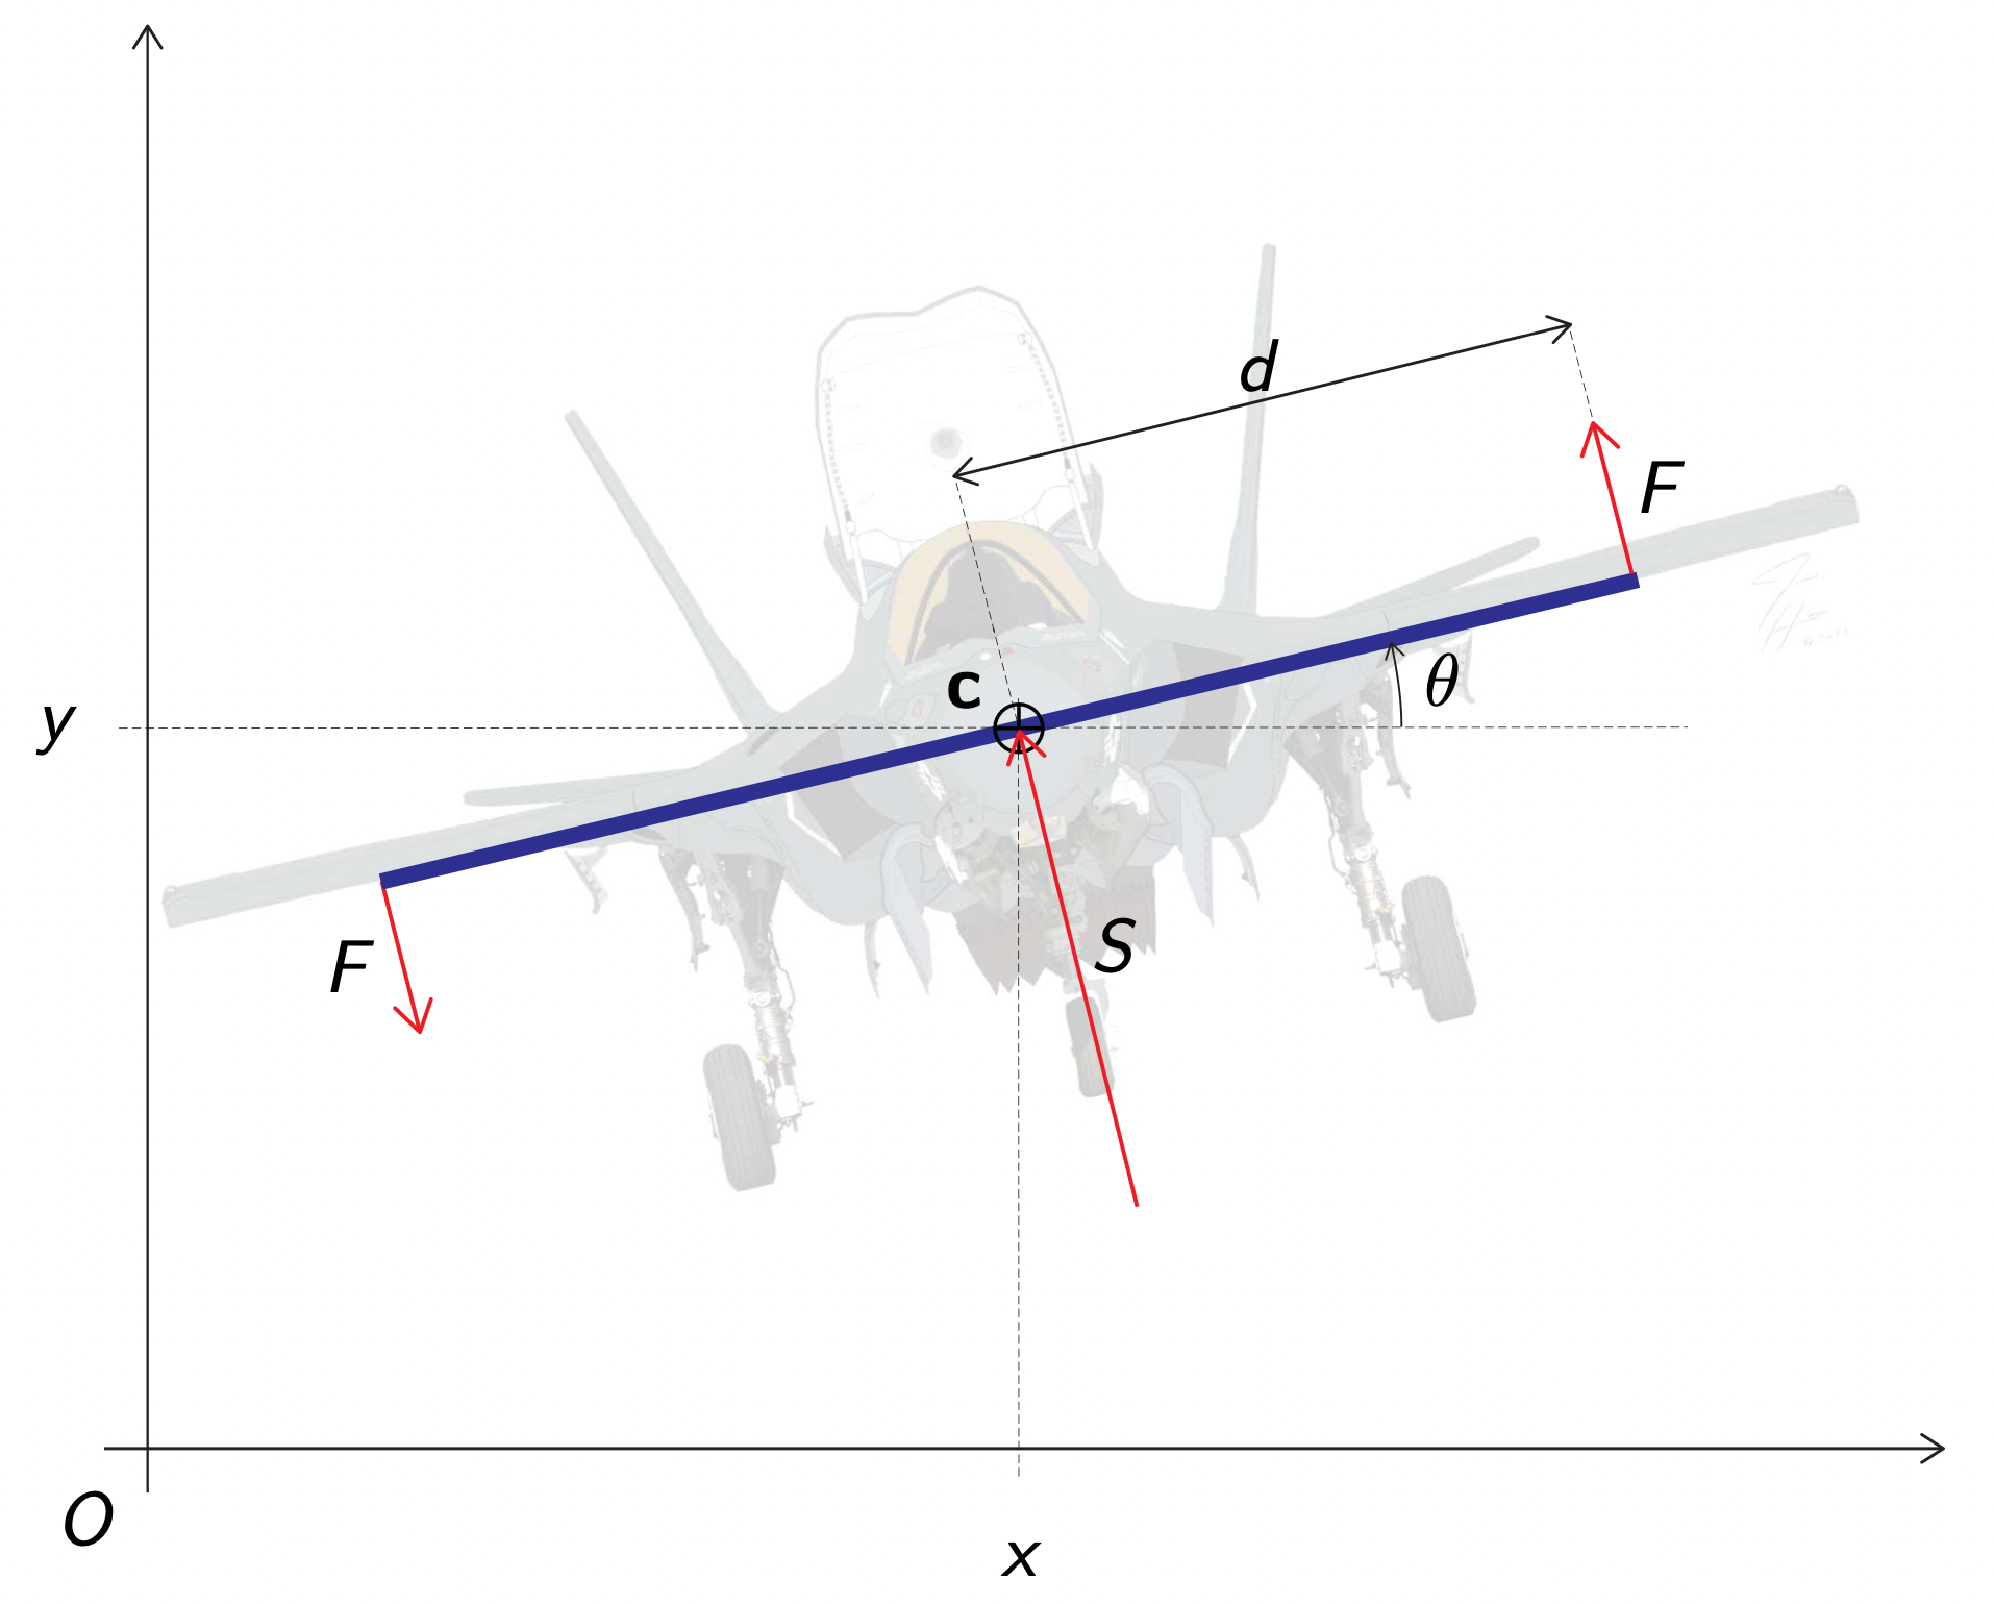
\includegraphics[width=0.75\columnwidth]{drawing}
}
\caption{Sketch of the system for aircraft vertical takeoff and landing.}
\label{fig:figure_2}
\end{figure}


\noindent
The dynamic model of this system is
\begin{eqnarray*}
\ddot{x}  &=&- \frac{1}{m}  \sin (\theta) S,\\
\ddot{y} &=&- g + \frac{1}{m} \cos ( \theta) S, \\
 \ddot{\theta} &=& \frac{2 d}{J}  F,
\end{eqnarray*}
with the following parameters 
\begin{itemize}
\item
barycentric moment of inertia of the aircraft: $J = 10 000 \; [\text{kg m}^2]$, 
\item
mass of the aircraft: $m = 30 000 \; [\text{kg}]$, 
\item
$d = 5.5 \; [\text{m}]$, 
\item
gravity acceleration: $g = 9.81 \; [\text{m}/\text{s}^2]$.
\end{itemize}


















\begin{itemize}

\item[1)] Demonstrate the equations of the dynamic model using the Lagrange method. (Copy the solution from Problem 1)

\item[2)] Calculate the state space representation of the system, assuming that $\mathbf{x} = (x, y, \theta, \dot{x}, \dot{y}, \dot{\theta})^T = ( x_1, x_2, x_3, x_4, x_5, x_6)^T$, where
distances are measured in [m], angles in [rad], linear velocities in [m/s], and angular velocities in [rad/s]. 
(Copy the solution from Problem 1)

\item[3)] Calculate all the operating points of the system and explain the obtained result.

\item[4)] Find the operating point that corresponds to $\overline{u}_1 = m g, \overline{u}_2 = 0$. Linearize the system around this operating point.

\item[5)] 
Is the linearized system controllable using both control inputs  $u_1$ and $u_2$? 
Is the linearized system controllable using only the control input $u_1$? 

\item[6)] Using the pole placement or the linear quadratic regulator method, design a state feedback controller to control the landing of the aircraft. 
We want to steer the aircraft from the state $\mathbf{x} = (x, y, \theta, \dot{x}, \dot{y}, \dot{\theta})^T = (1,5,0.0174533,-0.1,\linebreak -0.2,0.00174533)^T$ to the state $\mathbf{x} = (0, 2.4, 0, 0, 0, 0)^T$. 
Give the eigenvalues that have been assigned to the controlled system and illustrate the behaviour of the controller by plotting the relevant state and control variables and by a graphical animation. 


\item[7)] Using the pole placement or the linear quadratic regulator method, design a state feedback controller to control a lateral displacement of the aircraft. 
We want to steer the aircraft from the state $\mathbf{x} = (x, y, \theta, \dot{x}, \dot{y}, \dot{\theta})^T = (0,5,0.0174533,\linebreak -0.1,-0.2,0.00174533)^T$ to the state $\mathbf{x} = (10, 5, 0, 0, 0, 0)^T$. 
Give the eigenvalues that have been assigned to the controlled system and illustrate the behaviour of the controller by plotting the relevant state and control variables and by a graphical animation. 


\end{itemize}

\bigskip

\noindent
{\color{red} Write a detailed report answering each question in a different section. 

\bigskip

\noindent
Originality and completeness of the answers will be the aspects that will be taken into account in the grading of the report. Include the Matlab code in the report.

\bigskip

\noindent
 Additionally, upload the Matlab code to Aula Virtual. Upload the code of each answer in a separate folder. 
} 



\newpage

\section*{Solution of Pr\'actica 2}


\begin{itemize}

\item[1)] 
{\color{gray}
Demonstrate the equations of the dynamic model using the Lagrange method. (Copy the solution from Problem 1)
}

\bigskip

Mediante el metodo de Lagrange hallamos las ecuaciones de estado del modelo dinamico, sabiendo que: L = T - V\\\\
		$L = \frac{1}{2}(m(\dot{x}^2+\dot{y}^2)+J\dot{\theta}^2) - mgy$\\

Por tanto, las ecuaciones de Lagrange son las siguientes:\\\\
		$\frac{d}{dt}\frac{\partial L}{\partial \dot{x}} - \frac{\partial L}{\partial x} = S$\\\\
		$\frac{d}{dt}\frac{\partial L}{\partial \dot{y}} - \frac{\partial L}{\partial y} = S$\\\\
		$\frac{d}{dt}\frac{\partial L}{\partial \dot{\theta}} - \frac{\partial L}{\partial \theta} = F$\\\\

Tanto en la primera ecuacion como en la segunda, se iguala a la fuerza de empuje aplicada al centro de masas, mientras que en la tercera, se iguala a la fuerza aplicada en las puntas de las alas.\\

Resolvemos la primera ecuacion\\\\
		$\frac{\partial L}{\partial \dot{x}} = m\dot{x}$\\\\
		$\frac{d}{dt}\frac{\partial L}{\partial \dot{x}} = m\ddot{x}$\\\\
		$\frac{\partial L}{\partial x} = 0$\\\\
obteniendo la primera ecuacion de Lagrange:\\\\
		$m\ddot{x} = -S sen(\theta)$.\\

De la misma manera\\\\
		$\frac{\partial L}{\partial \dot{y}} = m\dot{y}$\\\\
		$\frac{d}{dt}\frac{\partial L}{\partial \dot{y}} = m\ddot{y}$\\\\
		$\frac{\partial L}{\partial y} = -mg$\\\\
obtenemos la segunda ecuacion de Lagrange: \\\\
		$m(\ddot{y} + g) = S cos(\theta)$.\\\\
Por último\\\\
		$\frac{\partial L}{\partial \dot{\theta}} = J\dot{\theta}$\\\\
		$\frac{d}{dt}\frac{\partial L}{\partial \dot{\theta}} = J\ddot{\theta}$\\\\
		$\frac{\partial L}{\partial \theta} = 0$\\\\
obtenemos la tecera y última ecuacion de Lagrange:\\\\
		$J\ddot{\theta} = F2d$.\\\\
En esta última multiplicamos la fuerza por 2d dado que es la distancia total entre la punta de una ala y la otra.\\\\Tal como podemos comprobar, dichas ecuaciones coinciden con las que teniamos que demostrar.

\bigskip




\item[2)] 
{\color{gray}
Calculate the state space representation of the system, assuming that $\mathbf{x} = (x, y, \theta, \dot{x}, \dot{y}, \dot{\theta})^T = ( x_1, x_2, x_3, x_4, x_5, x_6)^T$, where
distances are measured in [m], angles in [rad], linear velocities in [m/s], and angular velocities in [rad/s]. 
(Copy the solution from Problem 1)
}

\bigskip

Asumiendo que:\\\\
		$x = 
			\begin{pmatrix}
				 x_1\\x_2\\x_3\\x_4\\x_5\\x_6
			\end{pmatrix}
		 		= 
			\begin{pmatrix}
				 x\\y\\\theta\\\dot{x}\\\dot{y}\\\dot{\theta}
			\end{pmatrix}$,\\\\
podemos escribir:\\\\
		$\frac{d}{dt}
			\begin{pmatrix}
				 x\\y\\\theta\\\dot{x}\\\dot{y}\\\dot{\theta}
			\end{pmatrix}
				=
			\begin{pmatrix}
				 \dot{x}\\\dot{y}\\\dot{\theta}\\\ddot{x}\\\ddot{y}\\\ddot{\theta}
			\end{pmatrix}
				=
			\begin{pmatrix}
				 \dot{x}\\\dot{y}\\\dot{\theta}\\-\frac{1}{m}\sin(\theta)S\\-g+\frac{1}{m}\cos (\theta)S\\\frac{2d}{J}F
			\end{pmatrix}$.\\\\
Por tanto, la representacion del espacio de estados es:\\\\
	$\dot{x_1}=x_4$,\\
	$\dot{x_2}=x_5$,\\
	$\dot{x_3}=x_6$,\\
	$\dot{x_4}=-\frac{1}{m}\sin(\theta)S$,\\
	$\dot{x_5}=-g+\frac{1}{m}\cos (\theta)S$,\\
	$\dot{x_6}=\frac{2d}{J}F$\\	


\bigskip

\item[3)] 
{\color{gray}
Calculate all the operating points of the system and explain the obtained result.
}

\bigskip

Resolvemos la ecuacion $f(\bar{x},\bar{u}) = 0$. La solucion de dicha ecuacion seran los puntos de operacion.

\bigskip

\begin{tcolorbox}
[
%width=12cm,
title={File \texttt{answer\_3.m}}      
]
\begin{scriptsize}
\begin{verbatim}

close all;
clear all;
clc;

syms x1 x2 x3 x4 x5 x6 u1 u2 m d g J

S = solve(x4 == 0, x5 == 0, x6 == 0, (-1/m)*sin(x3)*u1==0,
	-g + (1/m)*cos(x3)*u1==0, (2*d/J)*u2==0,'Real', true)

\end{verbatim}
\end{scriptsize}
\end{tcolorbox}

\bigskip

A continuacion se muestran los puntos de operacion obtenidos: $u_1: g*m, u_2: 0, x_3: 0, x_4: 0, x_5: 0, x_6: 0$.

\bigskip

\item[4)] 
{\color{gray}
Find the operating point that corresponds to $\overline{u}_1 = m g, \overline{u}_2 = 0$. Linearize the system around this operating point.
}

\bigskip

Para linealizar el sistema en un punto operativo, es necesario que las ecuaciones del sistema tengan la siguiente forma:\\
	$\dot{x} = f(\bar{x},\bar{u}) + A(x-\bar{x}) + B(u-\bar{u})$\\
	$y = f(\bar{x},\bar{u}) + C(x-\bar{x}) + D(u-\bar{u})$\\
	
Para hallar las matrices A y B, es necesario hallar las derivadas parciales de $f(\bar{x},\bar{u})$. Dicho calculo lo realizamos mediante matlab con el uso del comando \textit{jacobian}.

\bigskip


\begin{tcolorbox}
[
%width=12cm,
title={File \texttt{answer\_4.m}}    
]
\begin{scriptsize}
\begin{verbatim}

close all;
clear all;
clc;

syms x1 x2 x3 x4 x5 x6 u1 u2 m d g J

f1 = x4;
f2 = x5;
f3 = x6;
f4 = (-1/m)*sin(x3)*u1;
f5 = -g + (1/m)*cos(x3)*u1;
f6 = (2*d/J)*u2;

A = jacobian([f1,f2,f3,f4,f5,f6], [x1,x2,x3,x4,x5,x6]);
B = jacobian([f1,f2,f3,f4,f5,f6], [u1,u2]);

A = subs(A, [m d g J x3 u1 u2], [30000 5.5 9.81 10000 0 30000*9.81 0])
B = subs(B, [m d g J x3 u1 u2], [30000 5.5 9.81 10000 0 30000*9.81 0])

C = jacobian([x1,x2], [x1,x2,x3,x4,x5,x6])


\end{verbatim}
\end{scriptsize}
\end{tcolorbox}

\bigskip

Una vez realizados los calculos:\\
	\begin{equation}A = 
		\begin{pmatrix}
		0 & 0 & 0 & 1 & 0 & 0\\
    		0 & 0 & 0 & 0 & 1 & 0\\
    		0 & 0 & 0 & 0 & 0 & 1\\
    		0 & 0 & -981/100 & 0 & 0 & 0\\
		0 & 0 & 0 & 0 & 0 & 0\\
    		0 & 0 & 0 & 0 & 0 & 0
		\end{pmatrix}
	\end{equation}
	
	\begin{equation}B = 
		\begin{pmatrix}
		0 & 0\\
    		0 & 0\\
    		0 & 0\\
    		0 & 0\\
    		1/30000 & 0\\
    		0 & 11/10000
		\end{pmatrix}
	\end{equation}
	
	\begin{equation}C = 
		\begin{pmatrix}
		1 & 0 & 0 & 0 & 0 & 0\\
     		0 & 1 & 0 & 0 & 0 & 0
		\end{pmatrix}
	\end{equation}\\
	
Por último, cabe destacar que la matriz C se define según los puntos del sistema que queramos observar. En este caso nos interesa las variables de estado x e y.

\bigskip

\item[5)] 
{\color{gray}
Is the linearized system controllable using both control inputs  $u_1$ and $u_2$? 
Is the linearized system controllable using only the control input $u_1$? 
}

\bigskip

El sistema linealizado es controlable usando ambas entradas de control $u_1$ y $u_2$ porque según el criterio de controlabilidad, Co tiene un rango total igual al rango de la matriz A, por ello la resta entre dichos rangos es 0, verificando dicho criterio.\\

El sistema también sería controlable unicamente con input $u_1$, ya que $u_2$ como en el ejemplo anterior seria nulo por lo que no afectaría al sistema.

\bigskip


\begin{tcolorbox}
[
%width=12cm,
title={File \texttt{answer\_5.m}}    
]
\begin{scriptsize}
\begin{verbatim}

close all;
clear all;
clc;

A =[0,0,0,1,0,0;
    0,0,0,0,1,0;
    0,0,0,0,0,1;
    0,0,-981/100,0,0,0;
    0,0,0,0,0,0;
    0,0,0,0,0,0];

B =[0,0;
    0,0;
    0,0;
    0,0;
    1/30000,0;
    0,11/10000];

Co = ctrb(A,B);

unco = length(A) - rank(Co)

\end{verbatim}
\end{scriptsize}
\end{tcolorbox}

\item[6)] 
{\color{gray}
Using the pole placement or the linear quadratic regulator method, design a state feedback controller to control the landing of the aircraft. 
We want to steer the aircraft from the state $\mathbf{x} = (x, y, \theta, \dot{x}, \dot{y}, \dot{\theta})^T = (1,5,0.0174533,-0.1,\linebreak -0.2,0.00174533)^T$ to the state $\mathbf{x} = (0, 2.4, 0, 0, 0, 0)^T$. 
Give the eigenvalues that have been assigned to the controlled system and illustrate the behaviour of the controller by plotting the relevant state and control variables and by a graphical animation. 
}

\bigskip

Para diseñar el controlador del avion emplearemos el algoritmo RegulNL.\\
Es necesario escoger una serie de polos para el controlador, por lo tanto los polos escogidos son -2,-2.1,-2.2,-1.2,-1.3 y -1.4. Posteriormente, calculamos $K = place(A,B,p_con)$ y $H = -(E(A-BK)^{-1}B)^{-1}$. Por último, el controlador se compone por la siguiente ecuacion:\\
	$u = \bar{u} - Kx + H(w - \bar{w})$\\
	
Por ultimo, para simular el sistema empleamos Euler.
\bigskip


\begin{tcolorbox}
[
%width=12cm,
title={File \texttt{answer\_6\_init.m}}   
]
\begin{scriptsize}
\begin{verbatim}

close all; 
clear all; 
clc;

figure
grid
hold

xmin=0;
xmax=15;
ymin=-5;
ymax=8;

axis([xmin xmax ymin ymax]); 
axis ('square');

\end{verbatim}
\end{scriptsize}
\end{tcolorbox}

\begin{tcolorbox}
[
%width=12cm,
title={File \texttt{answer\_6\_f.m}}      
]
\begin{scriptsize}
\begin{verbatim}

function  xdot  = p2_6_system_f(x,u)
% state x
% control u
x3 = x(3);
x4 = x(4);
x5 = x(5);
x6 = x(6);

u1 = u(1);
u2 = u(2);

m=30000;
g=9.81;
d = 5.5;
J = 10000;

xdot = [x4; x5; x6;
    (-1/m)*sin(x3)*u1;
    -g + (1/m)*cos(x3)*u1;
    (2*d/J)*u2];
end


\end{verbatim}
\end{scriptsize}
\end{tcolorbox}

\begin{tcolorbox}
[
%width=12cm,
title={File \texttt{answer\_6\_draw.m}}      
]
\begin{scriptsize}
\begin{verbatim}

function draw_plane(x,u)
    clf();
    d=5.5;
    u1=u(1);
    u2=u(2);
    hold on;
    axis square
    axis([-8,18,-10,10]);
    grid;
    
    P_ala_derecha_x = d*cos(x(3))+x(1);
    P_ala_derecha_y = d*sin(x(3))+x(2);
    P_ala_izquierda_x = -d*cos(x(3))+x(1);
    P_ala_izquierda_y = -d*sin(x(3))+x(2);
    
    % Representacion de fuerzas
    plot([P_ala_derecha_x, P_ala_derecha_x+u2*sin(x(3))],
    	[P_ala_derecha_y,-u2*cos(x(3))+P_ala_derecha_y], 'red', 'LineWidth',2);
    plot([P_ala_izquierda_x,P_ala_izquierda_x-u2*sin(x(3))],
    	[P_ala_izquierda_y,u2*cos(x(3))+P_ala_izquierda_y], 'red', 'LineWidth',2);
    plot([x(1), x(1)+u1*sin(x(3))], [x(2),-u1*cos(x(3))], 'red', 'LineWidth',2);
    
    % Representacion de las alas del avion
    plot([P_ala_derecha_x,P_ala_izquierda_x],
    	[P_ala_derecha_y,P_ala_izquierda_y], 'blue', 'LineWidth',2);
    
end

\end{verbatim}
\end{scriptsize}
\end{tcolorbox}


\begin{tcolorbox}
[
%width=12cm,
title={File \texttt{answer\_6\_main.m}}      
]
\begin{scriptsize}
\begin{verbatim}

init_6;

m = 30000;
g = 9.81;

dt=0.01;

A =[0,0,0,1,0,0;
    0,0,0,0,1,0;
    0,0,0,0,0,1;
    0,0,-981/100,0,0,0;
    0,0,0,0,0,0;
    0,0,0,0,0,0];

B =[0,0;
    0,0;
    0,0;
    0,0;
    1/30000,0;
    0,11/10000];

C = [1 0 0 0 0 0;
     0 1 0 0 0 0];

E = [1 0 0 0 0 0;
     0 1 0 0 0 0]; % Seleccion de las variables de estados que queremos controlar

Pcontrol = [-2,-2.1,-2.2,-1.2,-1.3,-1.4]; % Polos del controlador

K = place(A,B,Pcontrol);

H = -inv(E*inv(A-B*K)*B);

frame_counter=0;

x = [1;5;0.0174533;-0.1;-0.2;0.00174533]; % Estado inicial del sistema
t=0;
w = [0;2.4]; % Setpoint, a dónde queremos llegar

Ubarra = [m*g;0];

for t=0:dt:15

    u = Ubarra - K*(x-0)+H*(w-0); % Del algoritmo RegulNL
    w = [0;2.4];

    x = x + p2_6_system_f(x,u)*dt; % Euler
    
    pause(dt);
    
    frame_counter = frame_counter+1;
    
    % Frame sampling
    if frame_counter == 5
       u1 = u(1)/100000;
       u2 = u(2)/10;
       u = [u1;u2];
       draw_plane(x,u)
       %plot(t,x(1),'k--.',t,x(2),'r--.',t,x(3),'y--.', t,u1,'g--.', t,u2,'b--.')
       frame_counter =0;
    end
end
%legend('x','y','theta','S','F')

\end{verbatim}
\end{scriptsize}
\end{tcolorbox}

\bigskip
\begin{figure}[H]
\centerline{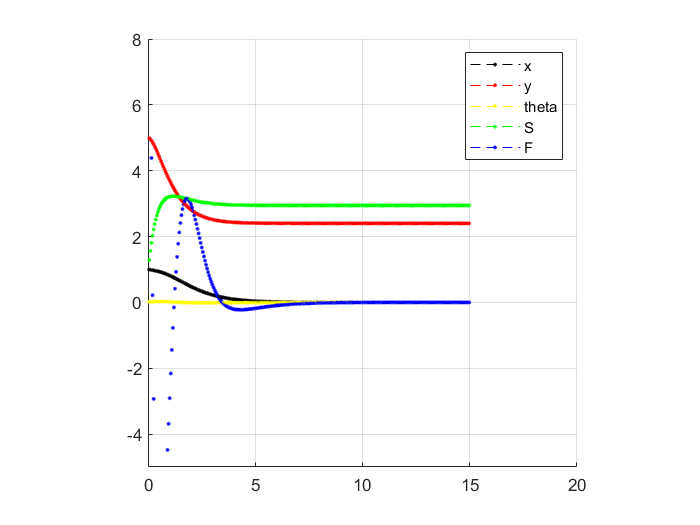
\includegraphics[scale=0.65]{figures/p2_6graphic}}
\caption{System State Variables Plot.}
\label{fig:figure2}
\end{figure}

\begin{figure}[H]
\centerline{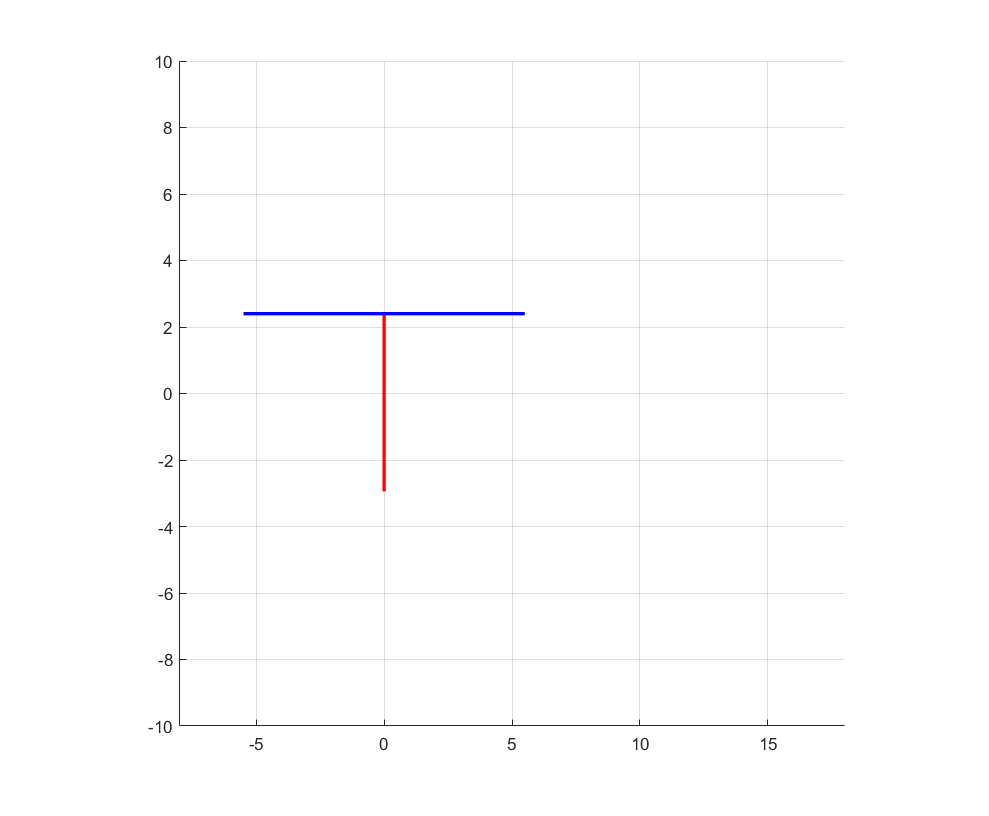
\includegraphics[scale=0.65]{figures/p2_6simulation}}
\caption{Simulation of the plane system.}
\label{fig:figure2}
\end{figure}
\bigskip

\item[7)] 
{\color{gray}
Using the pole placement or the linear quadratic regulator method, design a state feedback controller to control a lateral displacement of the aircraft. 
We want to steer the aircraft from the state $\mathbf{x} = (x, y, \theta, \dot{x}, \dot{y}, \dot{\theta})^T = (0,5,0.0174533,\linebreak -0.1,-0.2,0.00174533)^T$ to the state $\mathbf{x} = (10, 5, 0, 0, 0, 0)^T$. 
Give the eigenvalues that have been assigned to the controlled system and illustrate the behaviour of the controller by plotting the relevant state and control variables and by a graphical animation. 
}

\bigskip

Al igual que en el apartado anterior, seguiremos la misma estructura y emplearemos el algoritmo RegulNL. Sin embargo, los polos escogidos para este caso son -0.5,-2.2,-2,-2.3,-2.4 y -2.6. 

\bigskip


\begin{tcolorbox}
[
%width=12cm,
title={File \texttt{answer\_7\_init.m}}   
]
\begin{scriptsize}
\begin{verbatim}

close all; 
clear all; 
clc;

figure
grid
hold

xmin=0;
xmax=20;
ymin=-5;
ymax=8;

axis([xmin xmax ymin ymax]); 
axis ('square');

\end{verbatim}
\end{scriptsize}
\end{tcolorbox}

\begin{tcolorbox}
[
%width=12cm,
title={File \texttt{answer\_7\_f.m}}      
]
\begin{scriptsize}
\begin{verbatim}

function  xdot  = p2_7_system_f(x,u)
% state x
% control u
x3 = x(3);
x4 = x(4);
x5 = x(5);
x6 = x(6);

u1 = u(1);
u2 = u(2);

m=30000;
g=9.81;
d = 5.5;
J = 10000;

xdot = [x4; x5; x6;
    (-1/m)*sin(x3)*u1;
    -g + (1/m)*cos(x3)*u1;
    (2*d/J)*u2];
end



\end{verbatim}
\end{scriptsize}
\end{tcolorbox}

\begin{tcolorbox}
[
%width=12cm,
title={File \texttt{answer\_7\_draw.m}}      
]
\begin{scriptsize}
\begin{verbatim}

function draw_plane(x,u)
    clf();
    d=5.5;
    u1=u(1);
    u2=u(2);
    hold on;
    axis square
    axis([-8,18,-10,10]);
    grid;
    
    P_ala_derecha_x = d*cos(x(3))+x(1);
    P_ala_derecha_y = d*sin(x(3))+x(2);
    P_ala_izquierda_x = -d*cos(x(3))+x(1);
    P_ala_izquierda_y = -d*sin(x(3))+x(2);
    
    % Representacion de fuerzas
    plot([P_ala_derecha_x, P_ala_derecha_x+u2*sin(x(3))],
    	[P_ala_derecha_y,-u2*cos(x(3))+P_ala_derecha_y], 'red', 'LineWidth',2);
    plot([P_ala_izquierda_x,P_ala_izquierda_x-u2*sin(x(3))],
    	[P_ala_izquierda_y,u2*cos(x(3))+P_ala_izquierda_y], 'red', 'LineWidth',2);
    plot([x(1), x(1)+u1*sin(x(3))], [x(2),-u1*cos(x(3))], 'red', 'LineWidth',2);
    
    % Representacion de las alas del avion
    plot([P_ala_derecha_x,P_ala_izquierda_x],
    	[P_ala_derecha_y,P_ala_izquierda_y], 'blue', 'LineWidth',2);
    
end

\end{verbatim}
\end{scriptsize}
\end{tcolorbox}


\begin{tcolorbox}
[
%width=12cm,
title={File \texttt{answer\_7\_main.m}}      
]
\begin{scriptsize}
\begin{verbatim}

init_7;

m = 30000;
g = 9.81;

dt=0.01;

A =[0,0,0,1,0,0;
    0,0,0,0,1,0;
    0,0,0,0,0,1;
    0,0,-981/100,0,0,0;
    0,0,0,0,0,0;
    0,0,0,0,0,0];

B =[0,0;
    0,0;
    0,0;
    0,0;
    1/30000,0;
    0,11/10000];

C = [1 0 0 0 0 0;
     0 1 0 0 0 0];

E = [1 0 0 0 0 0;
     0 1 0 0 0 0]; % Seleccion de las variables de estados que queremos controlar

Pcontrol = [-0.5,-2.2,-2,-2.3,-2.4,-2.6]; % Polos del controlador

K = place(A,B,Pcontrol);

H = -inv(E*inv(A-B*K)*B);

frame_counter=0;

x = [0;5;0.0174533;-0.1;-0.2;0.00174533]; % Estado inicial del sistema
t=0;
w = [10;5]; % Setpoint, a dónde queremos llegar

Ubarra = [m*g;0];

for t=0:dt:20

    u = Ubarra - K*(x-0)+H*(w-0); % Del algoritmo RegulNL
    w = [10;5];

    x = x + p2_7_system_f(x,u)*dt; % Euler
    
    pause(dt);
    
    frame_counter = frame_counter+1;
    
    % Frame sampling
    if frame_counter == 5
       u1 = u(1)/100000;
       u2 = u(2)/10;
       u = [u1;u2];
       draw_plane(x,u)
       %plot(t,x(1),'k--.',t,x(2),'r--.',t,x(3),'y--.', t,u1,'g--.', t,u2,'b--.')
       frame_counter =0;
    end
end
%legend('x','y','theta','S','F')

\end{verbatim}
\end{scriptsize}
\end{tcolorbox}

\bigskip
\begin{figure}[H]
\centerline{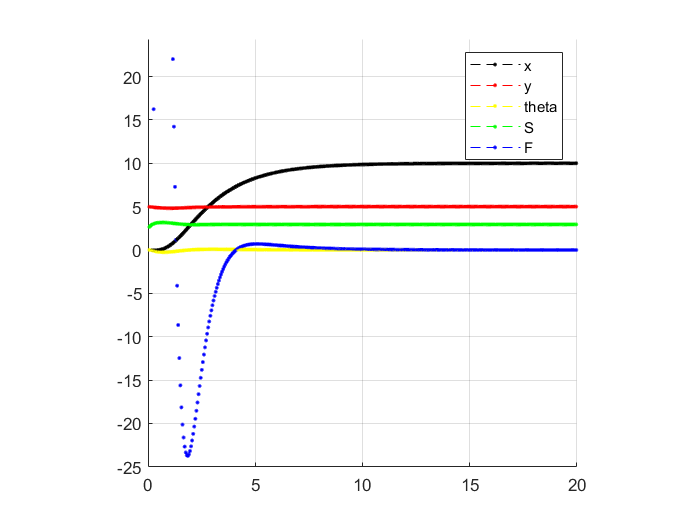
\includegraphics[scale=0.65]{figures/p2_7graphic}}
\caption{System State Variables Plot.}
\label{fig:figure2}
\end{figure}

\begin{figure}[H]
\centerline{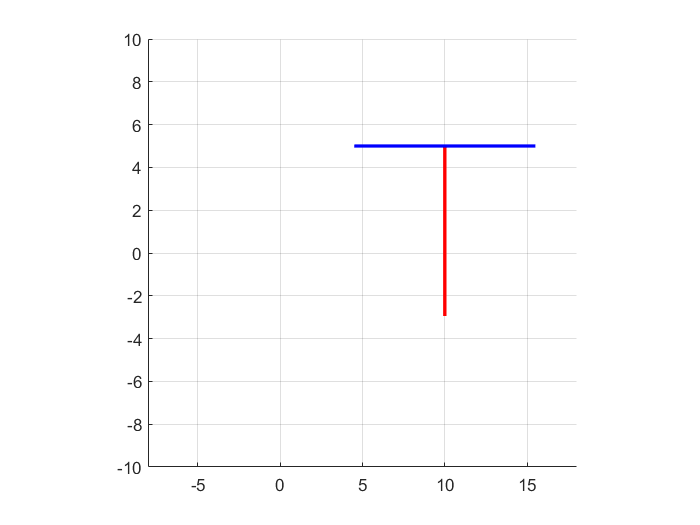
\includegraphics[scale=0.65]{figures/p2_7simulation}}
\caption{Simulation of the plane system.}
\label{fig:figure2}
\end{figure}
\bigskip

\end{itemize}

\end{document}
